\documentclass[11pt]{scrartcl}
\usepackage[T1]{fontenc}
\usepackage{selinput}
\usepackage[margin=2cm]{geometry}
\usepackage{enumitem,varwidth}
\usepackage[svgnames]{xcolor}
\usepackage{tikz}
\usetikzlibrary{shapes.geometric}
\usepackage{lmodern}

\parindent0em

\begin{document}

\section{SWOT Matrix - \emph{(Streghts, Weaknesses, Opportunities, Threats)}}

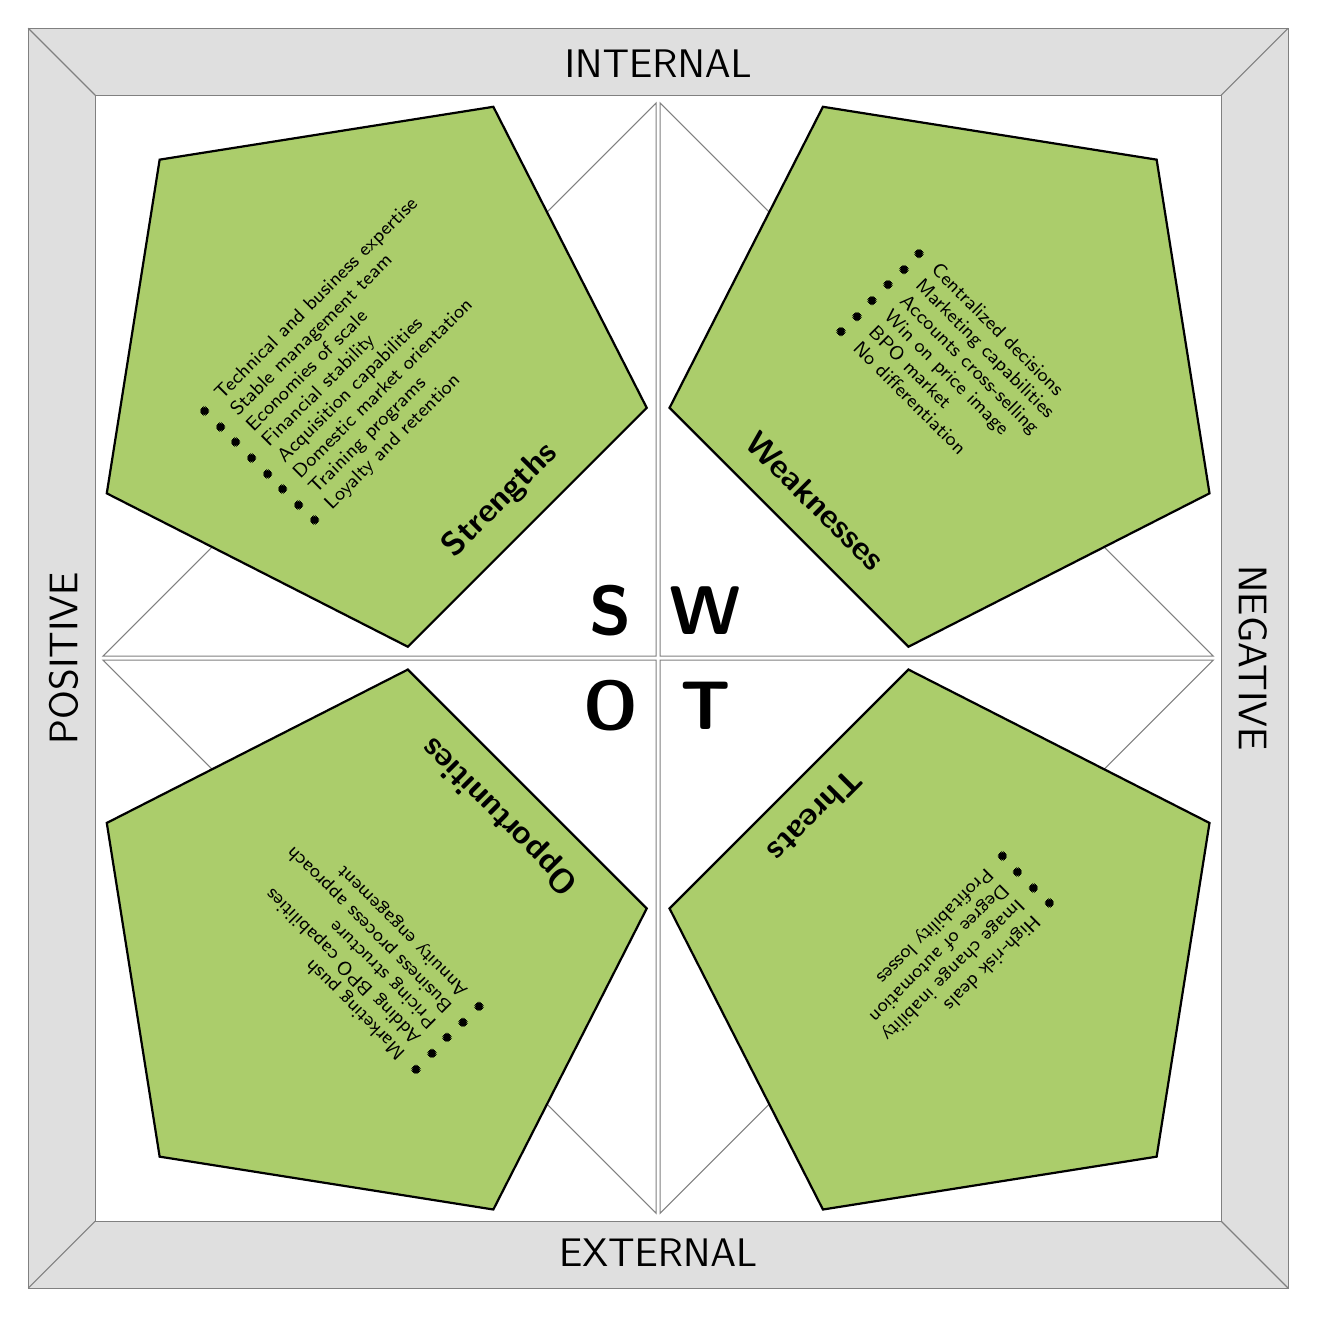
\begin{tikzpicture}[
    pentagon/.style={%
      shape=regular polygon,
      regular polygon sides=5,
      minimum size=7.3cm,
      inner sep=-1mm,
      draw,
      fill=DarkSeaGreen!75!yellow
    },
    font=\scriptsize\sffamily,
    thick
]

%    \draw[help lines] (-16,-16) grid (16,16);
\filldraw[thin,gray,fill=gray!25] (-8,-8) rectangle (8,8);
\filldraw[thin,gray,fill=white] (-7.15,-7.15) rectangle (7.15,7.15);
\draw[thin,gray] (7.15,7.15)--(8,8) (-7.15,7.15)--(-8,8) (-7.15,-7.15)--(-8,-8) (7.15,-7.15)--(8,-8);

% Strengths
\draw[thin,gray] (-0.025,0.025)--(-7.05,0.025)--(-0.025,7.05)--cycle;
\node[pentagon,rotate=45] at (-3.75,3.75) {
  \begin{varwidth}{\linewidth}
    \begin{itemize}[leftmargin=*,noitemsep]
      \item Technical and business expertise
      \item Stable management team
      \item Economies of scale
      \item Financial stability
      \item Acquisition capabilities
      \item Domestic market orientation
      \item Training programs
      \item Loyalty and retention
    \end{itemize}
  \end{varwidth}
};
\draw (-2,2) node[rotate=45] {\large\textbf{Strengths}};

% Weaknesses
\draw[thin,gray] (0.025,0.025)--(7.05,0.025)--(0.025,7.05)--cycle;
\node[pentagon,rotate=-45] at (3.75,3.75) {
  \begin{varwidth}{\linewidth}
    \begin{itemize}[leftmargin=*,noitemsep]
      \item Centralized decisions
      \item Marketing capabilities
      \item Accounts cross-selling
      \item Win on price image
      \item BPO market
      \item No differentiation
    \end{itemize}
  \end{varwidth}
};
\draw (2,2) node[rotate=-45] {\large\textbf{Weaknesses}};

% Opportunities
\draw[thin,gray] (-0.025,-0.025)--(-7.05,-0.025)--(-0.025,-7.05)--cycle;
\node[pentagon,rotate=135] at (-3.75,-3.75) {
  \begin{varwidth}{\linewidth}
    \begin{itemize}[leftmargin=*,noitemsep]
      \item Marketing push
      \item Adding BPO capabilities
      \item Pricing structure
      \item Business process approach
      \item Annuity engagement
    \end{itemize}
  \end{varwidth}
};
\draw (-2,-2) node[rotate=135] {\large\textbf{Opportunities}};

% Threats
\draw[thin,gray] (0.025,-0.025)--(7.05,-0.025)--(0.025,-7.05)--cycle;
\node[pentagon,rotate=-135] at (3.75,-3.75) {
  \begin{varwidth}{\linewidth}
    \begin{itemize}[leftmargin=*,noitemsep]
      \item High-risk deals
      \item Image change inability
      \item Degree of automation
      \item Profitability losses
    \end{itemize}
  \end{varwidth}
};
\draw (2,-2) node[rotate=-135] {\large\textbf{Threats}};
\draw(0,-7.55) node {\Large EXTERNAL};
\draw(0,7.55) node {\Large INTERNAL};
\draw(-7.55,0) node[rotate=90] {\Large POSITIVE};
\draw(7.55,0) node[rotate=270] {\Large NEGATIVE};
\draw(-0.6,0.6) node {\Huge\textbf{S}}; 
\draw(0.6,0.6) node {\Huge\textbf{W}};
\draw(-0.6,-0.6) node {\Huge\textbf{O}};
\draw(0.6,-0.6) node {\Huge\textbf{T}};
\end{tikzpicture}
  
\end{document}